\section{KHR}
\subsection{Vensl og eiginleikar þeirra (e. Relations and Their Properties)}
Finnum tvenndinar í venslunnm R úr A = \{0,1,2,3,4\} í B = \{0,1,2,3,4\}.\\ 
Þar sem $(a,b) \in R$ þá og því aðeins af.\\
A er formengi og B er bakmengi þar sem $A \rightarrow B$. Vansl eru alltaf rituð svona $(a,b) \in R$ þar sem fyrsta mengið (a) er formengið og seinna (b) bakmengi.\\

a) a = b og fáum: $R = \{(0,0), (1,1),(2,2),(3,3)\}$.\\ \hspace*{2.1em} Þetta eru allar leiðir sem a = b.\\

b)$a + b = 4$ og fáum $R = \{(1,3),(2,2),(3,1),(4,0)\}$.\\

c) lcm (a,b) = 2 og fáum $R = \{(1,2),(2,1),(2,2)\}$.\\ \hspace*{2.1em} Við skoðum þetta þannig að ef við erum með 1,2 þá er það $1^1 \quad \underline{2}^{\underline{1}}$ þar sem \hspace*{2.2em} við tökum stæra veldið og 2 og þar sem $2^1 = 2$ þá situm við það inn.
\subsubsection{Annað dæmi}
Ákvörðum hvort vensk R á mengi allra vefsíða séu spegilvirk, samhverf, andsamhverf og gegnvirk ef $(a,b) \in R$ þá og því aðeins af.\\
\textbf{Spegilvirk} Þíðir að allir eru venslaðir við sjálfan sig.\\
\textbf{Samhverf} Þíðir að ef $(a,b) \in R$ þá er $(b,a) \in R$ líka aka $(a,b) \in R \rightarrow (b,a) \in R$.\\
\textbf{Andsamhverf} Ef það virkar í báðar átir þá er a og b sama stak aka: \\$(aRb \wedge bRa) \rightarrow (a=b)$. Og bara í sömu átt.\\
\hbox{\textbf{Gegnvirk} Ef er venslað við b og b er venslað við c þá hlítur a að vera venslað við c.}\\
$((aRb) \wedge (bRc)) \rightarrow (aRc)$.\\


a) Allir sem hafa heimsótt a hafa heimsótt b. A er hlutmengi í B.\\
\hspace*{2.2em} Spegilvirk: Já því allir sem hafa heimsótt a hafa heimsótt a.\\
\hspace*{2.2em} Samhverf: Nei til dæmis gætu allir sem hafa heimsótt ruv.is heimsótt fb.com \hspace*{2.2em} en ekki öfugt.\\
\hspace*{2.2em} Andsamhverf: Nei til dæmis hefur fólk skoðað bloggið mitt og blogg bróðurs \hspace*{2.2em} míns. Það er samt ekki sama vefsíða.\\ 
\hspace*{2.2em} Gegnvirk: Já ef til eru þrjár vefsíður a, b og c þannig að allir sem skoðuð \hspace*{2.2em} a skoðuðu b og allir sem skoðuð b skoðuð líka c þá hlítur að vera að allir sem \hspace*{2.2em} skoðuðu a skoðuðu c.\\

\newpage
\subsubsection{Annað dæmi vensla}
Látum A vera mengi nemanda og B mengi bóka.\\
$aR_1B$: a á að lesa b fyrir skólan.\\
$aR_2B$: a er búin að lesa b.\\

a) $R_1 \cup R_2$: á að lesa eða búin að lesa.\\

b) $R_1 \cap R_2$: á að lesa og búin að lesa.\\

c) $R_1 \oplus R_2$: á að lesa en ekki búin eða á ekki að lesa en er búin.\\

d) $R_1 - R_2$: á að lesa en ekki búin.\\

e) $R_2 - R_1$: búin að lesa en áttir ekki að lesa.

\subsubsection{Annað dæmi vensla}
Látum R og S vera vensl á mengi fólks.\\
$aRb:$ a er foreldri b.\\
$aSb:$ a er systkin b.\\

Finnum $\underleftarrow{R\circ S} \text{ og } \underleftarrow{S\circ R}$: Lesið til vinstri.

$aR \circ Sc$: a er systkin b og b er foreldri c. ($aSb \wedge bRc$).

$aS \circ Rc$: a er foreldri c og c á systkin. ($aRb \wedge bSc$)

\newpage
\setcounter{subsection}{2}
\subsection{Framsetning vensla (e. Representing Relations)}

\subsubsection{Vensl framsetning með filki}
Ritum eftirfarandi vensl á mengið \{1,2,3\} sem fylki:\\
$R = \{(1,2), (2,1), (2,2), (3,3)\}$.\\
Fáum firkið:\vspace*{0.5em}\\ 
$M_R = \begin{bmatrix}
    0 & 1 & 0 \\
    1 & 1 & 0 \\
    0 & 1 & 1 \\
\end{bmatrix}$

\subsubsection{Vensl taling staka í filki}
Í fylki venslana R á $\{1,2,3,\ldots , 100\}$ er hversu margir ásar ef $(a,b) \in R$ þ.þ.a.a $a \geq b$. $R = \{(a,b)|a > b\}$.\vspace*{0.5em}\\
\(
\text{Skoðum }M_R = \bordermatrix{
    & 1 & 2 & 3 & \cdots & 99 & 100 \cr
    1 & 0 & 0 & 0 & \cdots & 0 & 0 \cr
    2 & 1 & 0 & 0 & \cdots & 0 & 0 \cr
    3 & 1 & 1 & 0 & \cdots & 0 & 0 \cr
    \vdots & \vdots & \vdots & \vdots & \ddots & \vdots & \vdots \cr
    99 & 1 & 1 & 1 & \cdots & 0 & 0 \cr
    100 & 1 & 1 & 1 & \cdots & 1 & 0 \cr
}
\)\vspace*{1em} \\
Af fylkinu sést að það eru $0,1,2,3 \ldots 99$ ásar í hveri línu. þá eru heildarfjöldi ása:\\
$\displaystyle \sum_{i=0}^{99}i = \frac{99 \cdot 100}{2} = 4950$ Það eru því 4950 ásar. 

\subsubsection{Vensl filki samsett vensk veldi}
Látum R vera vensl sem eru táknuð með fylkinu.\\
\(
M_R = \bordermatrix{
    & \cr
    & 0 & 1 & 0 \cr
    & 0 & 0 & 1 \cr
    & 1 & 1 & 0 
}
\)\vspace*{-1.5em}\\
a) Finnum $R^2$: Fáum $M_{R^2} \odot M_2$ \(
\bordermatrix{
    & \cr
    & 0 & 1 & 0 \cr
    & 0 & 0 & 1 \cr
    & 1 & 1 & 0 
}
\)
\(
\odot \bordermatrix{
    & \cr
    & 0 & 1 & 0 \cr
    & 0 & 0 & 1 \cr
    & 1 & 1 & 0 
}
\)= \hspace*{-1em}
\(
\bordermatrix{
    & \cr
    & 0 & 0 & 1 \cr
    & 1 & 1 & 0 \cr
    & 0 & 1 & 1 
} 
\)\\
b) Finnum $R^3$: Fáum $M_{R^3} \odot M_R$ \(
\bordermatrix{
    & \cr
    & 0 & 0 & 1 \cr
    & 1 & 1 & 0 \cr
    & 0 & 1 & 1 
}
\)
\(
\odot \bordermatrix{
    & \cr
    & 0 & 1 & 0 \cr
    & 0 & 0 & 1 \cr
    & 1 & 1 & 0 
}
\)= \hspace*{-1em}
\(
\bordermatrix{
    & \cr
    & 1 & 1 & 0 \cr
    & 0 & 1 & 1 \cr
    & 1 & 1 & 1 
} 
\)\vspace*{0.5em}\\
Hafa í huga að ef við erum með $S \odot R = M_R \odot M_S$ það verður öfugt.
\newpage
\subsubsection{Vensl framsetning með neti }
Finnum allar tvenndinar venslunum R sem er táknað með netinnu.\\

\begin{multicols}{2}
    Fáum: $R=\{(a,a),(a,b),(a,c),
    \\(b,a),(b,b),(b,c),(c,a),(c,b),(d,d)\}$
    \columnbreak
    \begin{center}
        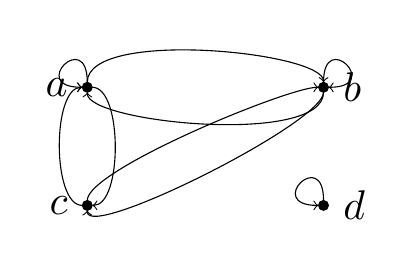
\begin{tikzpicture}[scale=1.5, transform shape]
            \tikzset{Bullet/.style={circle,draw,fill=black,scale=0.25}}
            \node[Bullet,label=left :{$a$}] (a) at (0,2) {} ;
            \node[Bullet,label=right:{$b$}] (b) at (2,2) {} ;
            \node[Bullet,label=left:{$c$}] (c) at (0,1) {} ;
            \node[Bullet,label=right:{$d$}] (d) at (2,1) {} ;
            \draw[->] (a) .. controls +(up:5mm) and +(up:3mm) ..(b) {};
            \draw[->] (b) .. controls +(down:5mm) and +(down:3mm) ..(a) {};
            \draw[->] (a) .. controls +(right:3mm) and +(right:3mm) ..(c) {};
            \draw[->] (c) .. controls +(left:3mm) and +(left:3mm) ..(a) {};
            \draw[->] (a) .. controls +(up:5mm) and +(left:5mm) ..(a) {};
            \draw[->] (c) .. controls +(up:3mm) and +(left:3mm) ..(b) {};
            \draw[->] (b) .. controls +(down:3mm) and +(down:3mm) ..(c) {};
            \draw[->] (d) .. controls +(up:5mm) and +(left:5mm) ..(d) {};
            \draw[->] (b) .. controls +(up:5mm) and +(right:5mm) ..(b) {};
        \end{tikzpicture}
    \end{center}
\end{multicols}
\setcounter{subsection}{4}
\subsection{Jafngildisvensl (e. Equivalence Relations)}
\subsubsection{Jafngildisvensl}
Jafngildisvensl eru spegilvirk, samhverf og gegnvirk verður að vera allt.\\

a) $\{(0,0), (0,2),(2,0),(2,3),(3,2),(3,3)\}$

Þau eru ekki spegilvirk en þau eru samhverf en ekki gegnvirk þannig þetta er \hspace*{1em} ekki jafngildisvensl\\

b) $\{(0,0), (1,1),(1,2),(2,1),(2,2),(3,3)\}$

Þau eru spegilvirk og samhverf þar sem við gerum fara fram og til baka og þau \hspace*{1em} eru gegnvirk þar sem við getum stti okkur laið í gegnum hnútana svo já það er \hspace*{1em} jafngildisvensl.
\newpage